\graphicspath{ {./img/TheFEM/} }
\chapter{Review of Boundary Value Problems}


\section{Boundary value problems}
In this section we will define a general initial boundary value problem (I-BVP). In the first part we will introduce the differential formulation given in terms of a set of governing equations and properly specified boundary conditions. The resulting equations are obtained after using a generalized balance law. Following this classical and well known approach we formally re-state these equations in the so-called strong form. Subsequently we re-write and prove an equivalent form of the balance law in the form of an integral representation highly friendly for a numerical solution. Since in the integral description of the problem the order of the derivatives in the field functions decreases by one, the resulting statement is called a weak formulation. 
%%
\subsection{Differential formulation-Generalized balance law}
Let $ds$ be a differential surface element; $\dd{V}$ a differential volume element; $u(\vb{x},t)$ a scalar (or vector) function of space and time.
The flux or rate of flow of the quantity $u(\vb x, t)$ through $\dd{S}$ at time $t$ is defined like
\[p(\vb x)\grad u \cdot \hat n \dd{S} \enspace ,\]
where $p(\vb x)$ is a positive function, assumed known and time independent. Similarly, the time rate of change of $u(\vb x, t)$ in an element $\dd{V}$ is given by
\[\rho (\vb x)\pdv{u}{t} \dd{V} \enspace ,\]
where once again $\rho (\vb x)$ is a known, given, time independent positive function. Additional effects occurring in the element $\dd{V}$ at the time time can be expressed like
\[H(\vb x, t)\dd{V} \equiv  - q(\vb x)u(\vb x, t) + \hat F(\vb x,t)\]
where $\hat F(\vb x, t) = \rho (\vb x)F(\vb x, t)$. In the above the term $q u$ represent internal effects due to changes proportional to $u$ while $\hat F(\vb x, t)$ are other external influences in the medium.

Balancing the internal and external changes yields
\[\int\limits_V \rho (\vb x)\pdv{u}{t}\dd{V} = \int\limits_S p(\vb x)\vb \grad u \cdot \hat n\dd{S}  + \int\limits_V H(\vb x, t)\dd{V} \enspace ,\]
or equivalently
\[\int\limits_V \rho (\vb x)\pdv{u}{t}\dd{V} = \int\limits_S p(\vb x)\vb \grad u \cdot \hat n\dd{S}   - \int\limits_V q(\vb x)u(\vb x, t)\dd{V}  + \int\limits_V \rho (\vb x)F(\vb x, t)\dd{V} \enspace .\]

Using the divergence theorem as
\[\int\limits_S p(\vb x) \grad u \cdot \hat n \dd{S}  = \int\limits_V \vb \div  (p\vb \grad u)\dd{V}\]
yields after substitution
\[\int\limits_V \left[\rho (\vb x)\pdv{u}{t} - \div (p(\vb x)\grad u) + q(\vb x)u(\vb x, t) - \rho (\vb x)F(\vb x, t)\right]\dd{V}  = 0\]
Assuming a continuous integrand, the arbitrariness of $V$ implies
\[\rho (\vb x)\pdv{u}{t} - \div(p(\vb x)\grad u) + q(\vb x)u(\vb x, t) - \rho (\vb x)F(\vb x, t) = 0\]

Letting
\[\mathcal{L} \equiv  - \div p(\vb x)\grad + q(\vb x)\]
the generalized set of partial differential equations can be written like
\begin{equation}
\rho(\vb x) \pdv{u(\vb x, t)}{t} + \mathcal{L}u(\vb x, t) = \rho (\vb x)F(\vb x, t) \enspace .
\label{eq:GenPDE}
\end{equation}

And they are categorized as:
\begin{itemize}
    \item Hyperbolic;
    \[\rho(\vb x) \pdv[2]{u(\vb x, t)}{t} + \mathcal{L}u(\vb x,t) = 0\]

    \item Parabolic; and
    \[\rho(\vb x) \pdv{u(\vb x,t)}{t} + \mathcal{L}u(\vb x, t) = 0\]

    \item Elliptic
    \[\mathcal{L}u(\vb x, t) = \rho (\vb x)F(\vb x, t) \enspace .\]
\end{itemize}

It can be shown that $\mathcal{L}$ satisfies the \emph{symmetry} condition
\[\int\limits_V \mathcal{L}(u)v\dd{V} =  \int\limits_V \mathcal{L}(v)u \dd{V}\]
and positive definiteness \cite{book:sepulveda_fismat, book:arfken}
\[\int\limits_V \mathcal{L}(u)u\dd{V}  > 0, \quad \forall u \enspace .\]

\subsection{Strong form}
Given $\rho(\vb x)$, $q(\vb x)$, $p(\vb x)$, $F(\vb x, t)$ and $\bar u$ find $u(\vb x , t):V \to \mathbb{R}$ such:
\[\rho(\vb x) \pdv{u}{t} - \div \left[p(\vb x) \grad u\right] + q(\vb x) u(\vb x, t) - \rho(\vb x) F(\vb x, t) = 0 \quad \forall \vb x \in V \]
and
\begin{align*}
    &u = \bar u \quad \forall \vb x \in S_u\\
    &p(\vb x)u_{,i} \hat n_i= B(\vb x,t)\quad \forall \vb x \in  S_t \enspace .
\end{align*}


In the FEM we will look for approximate solutions to $u$ subject to the following conditions:
\[u = \bar u \quad \forall \vb x \in S_u \quad \text{(Essential boundary conditions)}\] 
and
\[\int\limits_S \left(\pdv{u}{x_j}\right)^2 \dd{S} < \infty \enspace ,\]
which corresponds to the functions being square integrable. We will denote this space by $\mathbb{H}$ .

The space of functions satisfying the above two conditions will be denoted by $\zeta$ and termed the space of trial functions, formally defined like:
\[\zeta  = \left\{ u \mid u \in \mathbb{H},u = \bar u \quad \forall\vb x  \in S_u \right\}\]

On the other hand, to validate (or test) the correctness of the approximated or proposed trial functions $u$ it is also necessary to introduce test functions $w$ which are arbitrary except that they satisfy the following conditions:
\[w = 0\quad \forall \vb x \in S_u\] 
and
\[\int\limits_S \left(\pdv{w}{x_j}\right)^2 \dd{S} < \infty \enspace ,\]
which corresponds to the functions being square integrable. The space of functions satisfying the above two conditions will be denoted by $\pounds$ and termed the space of test functions, formally defined like:
\[\pounds  = \left\{w \mid w \in \mathbb{H},w = 0 \quad \forall \vb x \in S_u\right\}\]

\subsection{Weak form}
Given $\rho(\vb x)$, $q(\vb x)$, $p(\vb x)$, $F(\vb x, t)$ and $\bar u$ find $u(\vb x , t):V \to \mathbb{R}$ and $\forall w \in \pounds$ such:
\[\int\limits_V p(\vb x) u_{,i}\, w_{,i}\dd{V} - \int\limits_{S_t} B(\vb x, t)w \dd{S}  + \int\limits_V q(\vb x)u(\vb x, t)w\dd{V}  + \int\limits_V \rho(\vb x)\pdv{u}{t}w \dd{V} - \int\limits_V \rho(\vb x) F(\vb x, t)w\dd{V} = 0\]
and
\[u = \bar u\quad \forall\vb x \in S_u \enspace .\]

\subsection{Equivalence between the strong and weak forms}
\begin{multline}
    -\int\limits_V [p(\vb x)u_{,i}]_{,i}w \dd{V} + \int\limits_{S_t} [p(\vb x)u_{,i}] \hat n_i w\dd{S} - \int\limits_{S_t} B(\vb x, t)w\dd{S}\\
    + \int\limits_V q(\vb x)u(\vb x, t)w \dd{V}  + \int\limits_V \rho(\vec x)\pdv{u}{t}w\dd{V} - \int\limits_V \rho(\vb x)F(\vb x, t)w\dd{V} = 0 
\end{multline}

Grouping together common terms yields
\[\int\limits_V \left\{\rho(\vb x)\pdv{u}{t} - [p(\vb x)u_{,i}]_{,i} + q(\vb x)u(\vb x, t) - \rho(\vb x)F(\vb x, t)\right\} w\dd{V} + \int \limits_{S_t} \left\{[p(\vb x)u_{,i}]\hat n_i - B(\vb x, t) \right\} w\dd{S} = 0\]
from which
\[\rho(\vb x)\pdv{u}{t} - [p(\vb x)u_{,i}]_{,i} + q(\vb x)u(\vb x, t) - \rho(\vb x)F(\vb x, t) = 0\]
and
\[p(\vb x)u_{,i}\hat n_i = B(\vb x, t)  \quad\forall \vb x \in S_t \enspace .\]


\section{Brief review of the linearized theory of elasticity model}
Here we present a brief description of the boundary value problem governing the response of an elastic body. For a full discussion of the model and its mathematical aspects the reader is referred to \cite{shames1997elastic}.

The governing equations (in terms of stresses) stem from the principle of conservation of linear momentum and conservation of moment of linear momentum. The former leads to a set of 3 partial differential equations in the components of the stress tensor while the latter leads to the symmetries in the stress tensor.

\begin{equation} \label{eq:pde}
\begin{aligned}
&\sigma_{ij,j} + {f_i} = \rho\ddot{u}_i \quad \forall\ \vb{x} \in V,\, t \in \mathbb{R}^{+}\\
&\sigma_{ij}=\sigma _{ji}.
\end{aligned} 
\end{equation}

In \cref{eq:pde} $\sigma_{ij}$ is the stress tensor; $f_i$ is the vector of body forces; and $u_i$ is the displacements vector.

Denoting the tractions vector associated with a surface with normal direction $\hat{n}_{j}$ by $t_i^{\hat n}$ we have the complete BVP as follows:

\begin{equation} \label{eq:bcs}
t_i^{\hat n} = \sigma_{ij} \hat{n}_{j} \quad \forall \in \vb{x} \in S.
\end{equation}

\Cref{eq:pde} correspond to 6 equations with 12 unknowns (the 9 components of the stress tensor and the 3 components of the displacements vector ) and the system is undetermined. In order to have a solvable BVP we must introduce kinematic strain-displacement relations and a stress-strain law. In the case of infinitesimal theory of elasticity the strain-displacement relation is given by:

\begin{equation}\label{eq:kin}
\varepsilon_{ij} = \frac{1}{2}(u_{i,j} + u_{j,i})
\end{equation}

where the term $\epsilon_{ij}$ is the symmetric component of the displacements gradient tensor. The components of the strain tensor describe the distortions and changes in magnitude (volumetric changes) of the material point in the continuum model. Now the simplest stress-strain (constitutive) relationship is given by Hooke's law\footnote{Despite the name of \emph{law} used, this relation is not always valid, but is a good approximation for small strains.}

\begin{equation} \label{eq:Hooke}
\sigma_{ij} = 2\mu \varepsilon_{ij} + \lambda \varepsilon_{kk}\delta_{ij} \enspace .
\end{equation}

where $\mu$ and $\lambda$ are material constants. The problem involves now a total of 18 equations and 18 unknowns can be solved if subjected to properly specified boundary conditions.

\subsection*{Displacement formulation}
Substituting \cref{eq:kin} in \cref{eq:Hooke} and the result in \cref{eq:pde} yields after some manipulation:

\begin{equation} \label{eq:navier}
(\lambda  + \mu)u_{j,ij} + \mu u_{i,jj} + {f_i} = \rho \ddot{u}_i \quad \forall \vb{x} \in V,\, t \in \mathbb{R}^{+}.
\end{equation}

Since \cref{eq:navier} ( simultaneously describing equilibrium, kinematic relations and constitutive response) is a second order equation governing the displacement field possible boundary conditions are in terms of the variable itself or its first oder derivatives. For a well-possed problem the following is a set of valid boundary conditions: 

\begin{equation}\label{eq:Wellbcs}
\begin{split}
&t_i^{\hat n} = \sigma _{ij} \hat n_{ij} \quad \forall\ \vb{x} \in S_t\\
& {u_i} = \bar{u}_i \quad \forall \vb x \in S_u
\end{split}
\end{equation}

and where ${S_t} \cup {S_u} = S$ and ${S_t} \cap {S_u} = \emptyset $. 


In the particular case in which $u_i$ is not a function of time, we obtain the static version of the BVP, i.e,
\begin{equation}
\begin{split}
&\left(\lambda  + \mu \right)u_{j,ij} + \mu u_{i,jj} + {f_i} = 0 \quad \forall \vb{x} \in V \\
&t_i^{\hat n} = \sigma _{ij} \hat n_{ij} \quad \forall\ \vb{x} \in S_t\\
& {u_i} = \bar{u}_i \quad \forall \vb x \in S_u
\end{split}
\end{equation}

Notice that the tractions BC 
\[t_i^{\hat n} = \mu (u_{i,j} + u_{j,i}) \hat{n}_j + \lambda u_{k,k} \delta_{ij}\hat{n}_j \enspace ,\]

actually involves first order displacements derivative and as such it is a Neumann boundary condition on $u_i$.
%

\subsection{Equivalence between strong and weak forms}
\subsubsection{Strong form}
The strong form corresponds to the differential formulation of the problem, it is denoted by $\{ S \}$ and it reads:

Given $f_i$, $t_i^{\hat n}$ and ${\bar u_i}$ find ${u_i}:V \to \mathbb{R}$ such:
%
\begin{equation} \label{eq:navier_2}
\begin{split}
&(\lambda  + \mu)u_{j,ij} + \mu u_{i,jj} + f_i = 0 \quad \forall \vb{x} \in V \\
&t_i^{\hat n} = \sigma _{ij} \hat{n}_{ij} \quad \forall \vb{x} \in S_t\\
&u_i = \bar{u}_i \quad \forall \vb{x} \in S_u
\end{split}
\end{equation}

In \cref{eq:navier_2} the boundary conditions specified by the traction vector $t_i^{\hat n}$ correspond to the natural boundary conditions, while those specified in terms of the displacements vector $\bar u_i$ represent the essential boundary conditions.

\begin{itemize}
\item We are interested in developing methods to obtain approximate solutions to $\{S\}$.
\item The FEM is formulated starting from a statement equivalent to $\{ S \}$ in which we use trial functions until certain prescribed conditions are met.
\item We will look for solutions $u_i$ subject to the following conditions:
\begin{align*}
&u_i = \bar u_i \qquad \text{in} \qquad S_u\\
&\intL_S \left(\pdv{u_i}{x_j} \right)^2 dS < \infty
\end{align*}

\end{itemize}

The first condition corresponds to the satisfaction of the essential boundary condition, while the second corresponds to the functions being square integrable. The space of functions satisfying the above two conditions is denoted by $\varsigma$ and formally defined like
%
\[\varsigma = \left\{u_i\left| {u_i} \in H, {u_i} = \bar{u}_i \in S_u \right. \right\} \enspace .\]
%
On the other hand, in order to validate the introduced trial functions we also need testing functions $w_i$ also called in the FEM literature weighting or distribution functions. These functions are arbitrary apart from having to satisfy the following conditions:
%
\begin{align*}
&w_i = 0 \quad in \quad {S_u}\\
&\intL_S \left(\pdv{w_i}{x_j}\right)^2 dS < \infty
\end{align*}
%
In what follows we formally denote the space of these functions by $V$ and define it like
%
\[V = \left\{ w_i\left| w_i \in H, u_i = w_i=0 \in S_u \right. \right\} \enspace .\]

\subsubsection{Weak form}
Here we will show that the equilibrium statement represented in the differential formulation can be described in alternative forms. In such description the continuity requirement for the trial functions is weaker than in the strong form leading to the term "weak" statement. Here this alternative representation will be denoted like $\{W\}$ and it reads;

Given $f_i$, $t_i^{\hat n}$ and ${\bar u_i}$ find ${u_i}:V \to \mathbb{R}$ and $\forall {w_i} \in V$ such:

\[\intL_V \sigma _{ij} w_{i,j}\, dV - \intL_V f_i w_i\, dV  - \intL_{S_t} t_i^{\hat n} w_i\, dS = 0\]

\subsubsection*{Proof 1:}
Let $u_i \in \varsigma $ be a solution to $\{S\}$ and let $w_i \in V $. Forming the inner product of the equilibrium statement given in \cref{eq:pde} with $w_i$ and forcing the integral over the domain to be zero we have
%
\[\intL_V (\sigma_{ij,j} + f_i ){w_i}\, dV = 0 \enspace ,\]
%
expanding the terms in the integrand and integrating by parts the first term on the left we have
%
\[\intL_V \sigma _{ij,j} w_i\, dV + \intL_V f_i w_i\, dV = 0 \enspace .\]
\[ - \intL_V w_{i,j} \sigma _{ij}\, dV  + \intL_S \sigma _{ij} \hat{n}_j w_i\, dS  + \intL\limits_V w_i f_i\, dV = 0 \]

since $w_i \in V$ it follows that $w_i = 0$ in $S_u$ from which

\begin{equation}\label{eq:weak}
\intL_V \sigma _{ij} w_{i,j}\, dV - \intL_V f_i w_i\, dV  - \intL_{S_t} t_i^{\hat n} w_i\, dS = 0
\end{equation}

Now, considering that $u_i$ is solution of the strong form $\{S\}$ it must satisfy $u_i = \bar u_{i} \quad \in \quad S_u$ and as a result $u_i \in \varsigma$. On the other hand, since $u_i$ satisfies \cref{eq:weak} $\forall {w_i} \in V$ we have that $u_i$ satisfies the definition of weak solution specified in $\{ W \}$.

\subsubsection*{Proof 2:}
Let $u_i$ be a solution of $\{W\}$ and thus $u_i \in \varsigma$ which means that
\[u_i = \bar u_{i} \quad \in \quad S_u\]
and that it satisfies
\[\intL_V \sigma _{ij} w_{i,j}\, dV - \intL_V f_i w_i\, dV - \intL_{S_t} t_i^n w_i\, dS = 0 \enspace ,\]
integrating by parts,
\[-\intL_V \sigma_{ij,j} w_idV + \intL_S \sigma_{ij} n_j w_i dS  - \intL_V f_i w_i dV - \intL_{S_t} {t_i^n} w_i dS = 0\]

Since ${w_i} \in V$ we have that ${w_i}=0$ in $S_u$ and therefore
\[\intL_V w_i(\sigma_{ij,j} + f_i)dV + \intL_{S_t} w_i( \sigma_{ij} n_j - t_i^n )dS = 0 \]
from which
\begin{equation} \label{equil_2}
\begin{split}
&\sigma_{ij,j} + f_i = 0 \quad \vb{x} \in V \\
&t_i^n = \sigma_{ij} n_j \quad \forall \vb{x} \in S_t\\
&{u_i} = \bar{u}_i \quad \forall \vb{x} \in S_u
\end{split}
\end{equation}

which is once again the strong form of the problem given in \cref{eq:pde}.

\subsection{Simple wedge under self-equilibrated loads}
Consider the double wedge of side $\ell$ and internal angle $2 \phi$ shown in \cref{fig:WEDGE}. It is assumed to be contained in the $X-Y$ plane, with loading conditions satisfying a plane strain (or plane stress) idealization. The material is elastic with Lame constants $\lambda$ and $\mu$. The wedge is loaded by uniform tractions of intensity $S$ applied over its four faces in such a way that the wedge is self-equilibrated. We wish to find the closed-form elasticity solution for the stress, strain and displacement fields throughout the problem domain.
%
\begin{figure}[h]
\centering
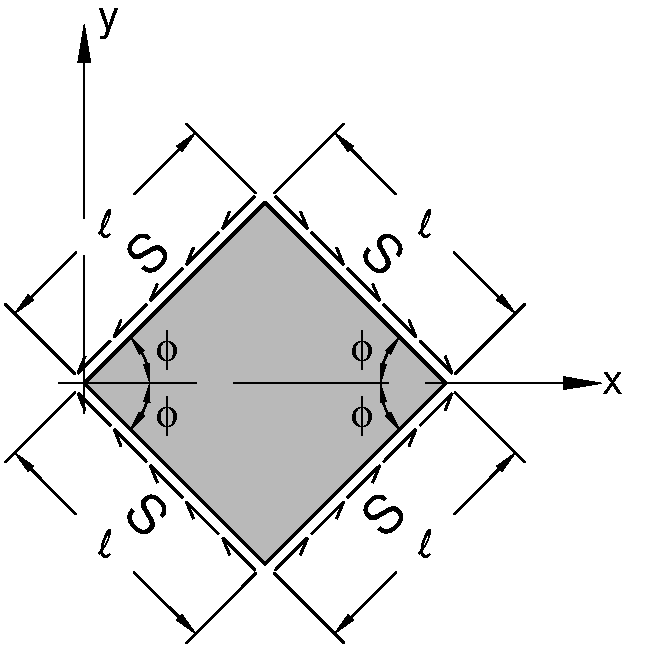
\includegraphics[width=7cm]{wedge.pdf}
\caption{2D Self-equilibrated wedge.}
\label{fig:WEDGE}
\end{figure}

Under plane strain conditions the general 3D stress equilibrium equations (see \cref{eq:pde}) reduce to:
\begin{equation}
\begin{aligned}
&\pdv{\sigma_{xx}}{x}+\pdv{\tau_{xy}}{y}=0\\
&\pdv{\tau_{xy}}{x}+\pdv{\sigma_{yy}}{y}=0
\end{aligned}
\label{eq:equilibrium}
\end{equation}

while the kinematic relation (\cref{eq:kin}) reads

\begin{equation}
\begin{aligned}
\epsilon_{xx}&=\pdv{u}{x}\\
\epsilon_{yy}&=\pdv{v}{y}\\
\gamma_{xy}&=\pdv{u}{y} + \pdv{v}{x}
\end{aligned}
\label{eq:strain}
\end{equation}
where $u$ and $v$ are the horizontal and vertical displacements respectively.

\subsubsection*{Stress field}

The stress field can be obtained by simple inspection from the traction boundary conditions prescribed over the inclined surfaces yielding;

\begin{align*}
\sum F_x &= 0 \longrightarrow - \ell S\cos(\phi)  + \sigma_{xx}\ell \sin(\phi) = 0\\
\sum F_y &= 0 \longrightarrow - \ell S\sin(\phi) - \sigma_{yy}\ell \cos(\phi)=0
\end{align*}

and the following stress solution:

\begin{equation}
\begin{aligned}
\sigma_{xx}& = S \cot(\phi)\\
\sigma_{yy}& = -S\tan(\phi)\\
\tau_{xy}& = 0.
\end{aligned}
\label{eq:solution}
\end{equation}

In \cref{eq:solution} the condition $\tau_{xy}=0$ is due to the symmetries in the problem.

\subsubsection*{Traction boundary conditions}
Let us verify that the above stress solution satisfies the traction BC using the expression:

\[t_i^{\hat n} = \sigma _{ij} \hat n_{ij}.\]

Denoting the outward normals to the inclined surfaces of the wedge by $\hat{n}^1$,  $\hat{n}^2$, $\hat{n}^3$, $\hat{n}^4$ these are given by;
\begin{align*}
\hat{n}^1 &= -\sin(\phi)\hat{e}_{x}+\cos(\phi)\hat{e}_{y}\\
\hat{n}^2 &= -\sin(\phi)\hat{e}_{x}-\cos(\phi)\hat{e}_{y}\\
\hat{n}^3 &= +\sin(\phi)\hat{e}_{x}+\cos(\phi)\hat{e}_{y}\\
\hat{n}^4 &= +\sin(\phi)\hat{e}_{x}-\cos(\phi)\hat{e}_{y} \enspace
\end{align*}

where $\hat{e}_{x}$ and $\hat{e}_{y}$ are the reference unit vectors. Now, the components of the traction vector follow directly like

\[t_{i} = \sigma_{ij}\hat{n}_{j}\]

then over the face with normal $\hat{n}^1$ we have
\begin{align*}
t_{x} &= -S\cos(\phi)\\
t_{y} &= -S\sin(\phi)
\end{align*}
similarly, over the face with normal $\hat{n}^2$
\begin{align*}
t_{x} &= -S\cos(\phi)\\
t_{y} &= +S\sin(\phi)
\end{align*}
over the face with normal $\hat{n}^3$ 
\begin{align*}
t_{x} &= +S\cos(\phi)\\
t_{y} &= -S\sin(\phi)
\end{align*}
and finally, over the face with normal $\hat{n}^4$;
\begin{align*}
t_{x} &= +S\cos(\phi)\\
t_{y} &= +S\sin(\phi) \enspace .
\end{align*}

\subsubsection*{Strain field}
The strain field can be obtained after using the stress solution found in \cref{eq:solution} together with the constitutive law given by \cref{eq:Hooke} which for a plane strain idealization takes the form:

\begin{equation}
\begin{aligned}
\epsilon_{xx}& = \frac{1}{E}(\sigma_{xx} - \nu \sigma_{yy}) \\
\epsilon_{yy}& = \frac{1}{E}(\sigma_{yy} - \nu \sigma_{xx}) \\
\gamma_{xy}& = \frac{\tau _{xy}}{\mu}
\end{aligned}
\label{eq:cons model}
\end{equation}

which for the particular case yields;


\begin{equation}
\begin{aligned}
\epsilon_{xx}& = +\dfrac{S}{E}\left[\cot(\phi)+\nu \tan(\phi)\right] = +\dfrac{S}{E}K_{1}(\nu , \phi)\\
\epsilon_{yy}& = -\dfrac{S}{E}\left[\tan(\phi)+\nu \cot(\phi)\right] = -\dfrac{S}{E}K_{2}(\nu , \phi)\\
\gamma_{xy}& = 0.
\end{aligned}
\label{eq:strain part}
\end{equation}

\subsubsection*{Displacement field}
The displacement field is obtained after direct integration of the strains after using the fact that:

\[du_i=\epsilon_{ij}dx_j + \omega_{ij}dx_j\]

and the condition $\omega_{xy}=0$ also due to symmetries , as follows:

\begin{align*}
u &= +\dfrac{S}{E} K_{1}(\nu , \phi)x + A\\
v &= -\dfrac{S}{E} K_{2}(\nu , \phi)y + B
\end{align*}

and where $A$ and $B$ are integration constants.

From the condition $u=0$ at $x=\ell\cos(\phi)$ we have that $A=-\dfrac{S}{E} K_{1}(\nu , \phi)\ell\cos(\phi)$ then it follows that
\[u=\dfrac{S}{E} K_{1}(\nu , \phi)(x-\ell\cos(\phi)).\]

Similarly, from the condition $v=0$ at $y=0$ we have that $B=0$ from which
\[v=-\dfrac{S}{E} K_{2}(\nu , \phi)y\]

\subsection{Variational formulation}
In this section we formulate the boundary value problem using the approach of the calculus of variations in which the governing PDEs and boundary conditions are obtained after finding the minimum (or maximum) of a functional according to a variational principle\footnote{According to Wikipedia \cite{wiki:variational_principle}

\begin{quotation}
A variational principle is a scientific principle used within the calculus of variations, which develops general methods for finding functions which minimize or maximize the value of quantities that depend upon those functions. For example, to answer this question: ``What is the shape of a chain suspended at both ends?" we can use the variational principle that the shape must minimize the gravitational potential energy.

According to Cornelius Lanczos, any physical law which can be expressed as a variational principle describes an expression which is self-adjoint. These expressions are also called Hermitian. Such an expression describes an invariant under a Hermitian transformation.
\end{quotation}}.

We will see that the weak form (and therefore also the strong form) can be obtained alternatively through the process of finding extreme values for a functional. We will illustrate this idea for the general case of theory of elasticity and then we will present particular examples.

\subsubsection*{Some vague definitions in the calculus of variations}
In variational calculus a {\bf functional} can be understood as a ``function" having as independent variables or arguments a space of vector functions and producing as a result (or dependent variable) a scalar. For instance, in the particular case of the theory of elasticity such a ``function" corresponds to the total potential energy functional $\Pi$ given by;
\begin{equation}\label{eq:Potential}
    \Pi(u_i) = \frac{1}{2}\int\limits_V \sigma_{ij}\varepsilon_{ij}\dd{V}  - \int\limits_V f_i\, u_i\dd{V}  - \int\limits_S t_i^{(n)} u_i\dd{S}
\end{equation}
and where the first term in the left hand side corresponds to the internal strain energy, while the last two terms are the work done by the external body and traction forces. The above functional has as independent variables the displacement vector and its spatial derivatives. This is indicated by the presence of the displacement vector $u_i$ in the expression $\Pi(u_i)$.

In variational calculus we are interested in finding a function $u_i$ that renders the functional $\Pi$ a maximum or a minimum. In loose terms, the analogous to the differential operator in calculus of functions is now termed the variational operator $\var$ (i.e., $\var$ is analogous to $\pdv{x_i}$). As such $\var{\Pi}$ acts over the function $u_i$ and its derivatives as follows
\[\var{\Pi}  = \pdv{\Pi}{u_i}\var{u_i} + \pdv{\Pi}{\left( \pdv{u_i}{x_j}\right)} \delta\left(\pdv{u_i}{x_j}\right) + \cdots + \pdv{\Pi}{\left( \pdv{^{n}u_i}{x_j \cdots \partial x_k}\right)} \delta\left( \pdv{^{n}u_i}{x_j \cdots \partial x_k}\right) \enspace .\]

The following rules apply to the variational operator $\delta$:
\begin{itemize}
\item For functionals $\Pi$ and $\Phi$ it follows that \[\var(\Pi  + \Phi) = \var{\Pi}  + \var{\Phi}\]
\item For functionals $\Pi$ and $\Phi$ it follows that \[\var(\Pi \Phi ) = \var{\Pi} \Phi  + \Pi \var{\Phi}\]
\item For a functional $\Pi$ and an integer $n$ it follows that \[\var(\Pi^n) = n(\Pi^{n - 1})\var{\Pi}\]
\item For a functional $\Pi$ it follows that \[\var{\int \Pi \dd{x}}  = \int \var{\Pi} \dd{x} \]
\end{itemize}

If the variational operator is applied to the functional $\Pi(u_i)$ it produces functions or variations in $u_i$ which are arbitrary and such $\var{u_i} \in V$ and $\var{u_i} = 0$ in $S_u$.

To find an extreme function in the calculus of variations we proceed like in differential calculus. Here we compute the first variation of the functional $\var{\Pi}$ and solve the variational equation
\begin{equation}\label{eq:vareq}
    \delta \Pi  = 0
\end{equation}
in the unknown function $u_i$. 

In the particular case of the total potential energy functional $\Pi$ this yields
\begin{equation}\label{eq:ClaPVW}
    \int\limits_V \sigma _{ij}\var{\varepsilon_{ij}}\dd{V}  - \int\limits_V f_i var{u_i} \dd{V}  - \int\limits_{S_t} t_i^{(n)} \var{u_i}\dd{S}  = 0
\end{equation}
where we recognize the weak form of the BVP stated previously. It becomes evident that the functions $\delta {u_i}$ in \cref{eq:ClaPVW} play the role of the test functions $w_i$ introduced in the weak form. On the other hand, since we have already shown that the weak and strong forms are equivalent we conclude that having the functional and the essential boundary conditions is equivalent to having the strong form of the problem.


\subsubsection*{Principle of minimum potential energy}
In the theory of elasticity the total potential energy $\Pi$ is the result of adding the elastic strain energy which is stored in the body upon deformation and the potential energy (work) imparted to the body by the applied forces. The principle states that the body is in equilibrium when this total potential energy reaches a minimum. This is equivalent to stating that an equilibrium configuration is attained when an infinitesimal variation from the position of minimum potential energy involves null changes in energy. This implies the variational condition:
\begin{equation}\label{vareq2}
    \delta \Pi  = 0.
\end{equation}

The above principle leads to the so-called principle of virtual displacements stated as follows\footnote{see Bathe pp 156}:
``The equilibrium of the body requires that for any compatible small virtual displacements satisfying the condition of being zero at $S_u$, imposed on the body in its state of equilibrium, the total internal virtual work is equal to the total external virtual work"
\[\int\limits_V \sigma _{ij}\var{\varepsilon_{ij}}\dd{V}  - \int\limits_V f_i\delta u_i\dd{V}  - \int\limits_{S_t} t_i^{(n)}\var{u_i}\dd{S}  = 0\]
where $\var{u_i}$ are the virtual displacements and $\var{ \varepsilon_{ij}}$ are the corresponding virtual strains.

Comparing the virtual work principle with the weak formulation given in \cref{eq:weak} we identify $\var{u_i}$ with the test functions $w_i$. As such the PVW takes the form of a powerful tool to test if a body is in equilibrium for a given solution (represented by the trial functions). In what follows we illustrate the use of the principle through some examples corresponding to problems in Bathe's textbook.

\subsubsection*{Problem\footnote{3.15 from Finite Element Procedures}}
Establish the differential equation of equilibrium of the problem shown and the boundary conditions. Determine whether the differential operator of the problem is symmetric and positive definite and prove your answer.\cite{book:bathe}

\begin{figure}[H]
    \centering
    \includegraphics[width=10cm]{{Bathe3.15}.pdf}
    \caption{Rod with varying cross-sectional area. The Young's modulus is E.}
    \label{fig:bathe3.15}
\end{figure}


\begin{align*}
\Pi &= \frac{1}{2}\int\limits_0^L \sigma_{xx}\varepsilon_{xx}A(x)\dd{x} + \frac{1}{2}ku_0^2 - R u_L \\
 &= \frac{1}{2}\int\limits_0^L EA(x)\left( \dv{u}{x}\right)^2 \dd{x} + \frac{1}{2}ku_0^2  - R u_L \enspace.
\end{align*}

The first variation for this functional is
\[\var{\Pi}  = \int\limits_0^L EA(x)\dv{u}{x}\dv{\var{u}}{x}\dd{x} + k u_0\var{u_0}  - R\var{u_L} \enspace .\]

If we integrate by parts, we obtain
\[\var{\Pi}  =  - \int\limits_0^L \dv{x}\left[EA(x)\dv{u}{x}\right]\var{u}\dd{x} + \left. EA(x)\dv{u}{x}\var{u} \right|_0^L + k{u_0}\var{u_0}  - R\var{u_L}\]
from which
\begin{align*}
&\dv{x}\left[EA(x)\dv{u}{x}\right] = 0\\
&\left. EA(x)\dv{u}{x}\right|_{x=0} = k u_0\\
&\left. EA(x)\dv{u}{x}\right|_{x=L} = R
\end{align*}


\subsubsection*{Problem: The Hu-Washizu Variational Principle\footnote{4.35 from Finite Element Procedures}}
Consider the Hu-Washizu functional:
\begin{equation}
\Pi^* = \Pi  - \intL_V \lambda_{ij}^\varepsilon (\varepsilon_{ij} - L_{ijk} u_k)\dd{V}  - \intL_{S_u} \lambda_i^u(u_i^{S_u} - \bar{ u}_i)\dd{S}
\label{eq:Hu}
\end{equation}

where
\begin{itemize}
\item $\Pi$: is the potential energy functional.
\item $L_{ijk}$ is a differential operator such $\varepsilon_{ij} = L_{ijk} u_k$.
\item $S_u$ surface where essential boundary conditions are prescribed.
\item $\lambda_{ij}^\varepsilon $ and $\lambda_i^u$ are Lagrange multipliers.
\end{itemize}

Using the condition $\var{\Pi} = 0$ derive for the interior of the body the equilibrium equations
\[\sigma_{ij,j} + f_i = 0\]
the strain-displacement relationship
\[\varepsilon_{ij} = L_{ijk} u_k\]
and the constitutive equation
\[\sigma_{ij} = C_{ijkl} \varepsilon_{kl}\]
and at the surface of the body the relation between the stress tensor and the applied tractions vector at $S_t$
\[t_i = \sigma_{ij} n_j\]
the relation between the stress tensor and the unknown tractions vector (or reactions) at $S_u$
\[t_i = \tilde{\sigma_{ij}} n_j\]
and the essential boundary condition at $S_u$
\[u_i = \tilde{u}_i\]
We want to determine the Euler equations resulting from the condition $\var{\Pi}^* = 0$. Applying the variational operator we have
\begin{equation}
\begin{aligned}
\var{\Pi}^*& = \var{\Pi}  - \intL_V \var{\lambda}_{ij}^{\varepsilon}  (\varepsilon_{ij} - L_{ijk} u_k)\dd{V}- \intL_V \lambda_{ij}^\varepsilon (\var{\varepsilon}_{ij} - L_{ijk}\var{u}_k)\dd{V} \\
&-\intL_V \var{\lambda}_i^u (u_i^{S_u} - \bar u_i)\dd{S} - \intL_V \lambda _i^u \var{u}_i^{S_u} \dd{S}
\end{aligned}
\end{equation}
and
\begin{equation}
\begin{aligned}
\var{\Pi}^* &= \intL_V C_{ijkl} \varepsilon_{kl} \var{ \varepsilon}_{ij}\dd{V} - \intL_{S_t} t_i \var{u_i} \dd{S}  - \intL_V f_i \var{u_i}\dd{V} - \intL_V \lambda_{ij}^{\varepsilon} \var{\varepsilon}_{ij}\dd{V}  + \intL_V \lambda_{ij}^{\varepsilon} L_{ijk}\var{u_k}\dd{V}\\
&- \intL_V \delta \lambda_{ij}^\varepsilon (\varepsilon_{ij} - L_{ijk} u_k)\dd{V} - \intL_S \var{\lambda}_i^u (u_i^{S_u} - \bar {u}_i)\dd{S} - \intL_{S_u} \lambda _i^u\var{u_i}\dd{S} = 0
\end{aligned}
\end{equation}
using
\[\intL_V (\lambda_{ij}^\varepsilon \var{u_i}){,_j}\dd{V} =  \intL_V \lambda_{ij}^\varepsilon \var{u}_{i,j}\dd{V}  + \intL_V \lambda_{ij,j}^\varepsilon \var{u_i}\dd{V} \]

In the above we can write
\begin{align*}
\intL_V \lambda_{ij}^\varepsilon L_{ijk}\var{u_k}\dd{V} & = \intL_V (\lambda_{ij}^\varepsilon \var{u_i})_{,j}\dd{V} - \intL_V \lambda_{ij,j}^\varepsilon \delta {u_i}\dd{V}\\
& = \intL_{S_t} \lambda_{ij}^\varepsilon \var{u_i}\hat {n}_j\dd{S}  - \intL_V \lambda_{ij,j}^\varepsilon \var{u_i}\dd{V}
\end{align*}
therefore
\begin{align*}
\delta \Pi^* &= \intL_V (C_{ijkl}\varepsilon_{kl} - \lambda_{ij}^\varepsilon) \var{\varepsilon}_{ij}\dd{V} - \intL_{S_t} t_i \var{u}_i\dd{S} - \intL_V f_i \var{u}_i\dd{V} + \intL_{S_t} \lambda_{ij}^\varepsilon \var{u_i}\hat{n}_j\dd{S}  - \intL_V \lambda_{ij,j}^\varepsilon \delta {u_i}\dd{V}\\
&- \intL_V \delta \lambda _{ij}^\varepsilon (\varepsilon_{ij} - L_{ijk} u_k)\dd{V}  - \intL_{S_u} \var{\lambda}_i^u (u_i^{S_u} - \bar{u}_i)\dd{S} - \intL_{S_u} \lambda_i^u \var{u_i} \dd{S}  = 0\\
&= \intL_V (C_{ijkl}\varepsilon_{kl} - \lambda_{ij}^\varepsilon) \var{\varepsilon}_{ij}\dd{V}
+ \intL_{S_t} (\lambda_{ij}^\varepsilon \hat{n}_j - t_i)\delta {u_i}\dd{S}\\
&- \intL_V (\lambda_{ij,j}^\varepsilon  + f_i) \var{u_i}\dd{V}
- \intL_V (\varepsilon_{ij} - L_{ijk} u_k) \var{\lambda} _{ij}^\varepsilon\dd{V}
- \intL_{S_u} (u_i^{S_u} - \bar{u}_i) \var{\lambda}_i^u\dd{S}  - \cancel{\intL_{S_u} \lambda _i^u \var{u}_i^{S_u}\dd{S}} = 0
\end{align*}

Now, imposing the conditions $\var{\varepsilon}_{ij} \neq 0$, $\var{\lambda}_{ij}^\varepsilon  \neq 0$, $var{u}_i \neq 0$ in $S_t$, $\var{u}_i \neq 0$ in $V$ and $\var{\lambda}_i^u \neq 0$ in $S_u$ we have
\begin{align}
&\lambda_{ij}^\varepsilon  = C_{ijkl} \varepsilon_{kl}\\
&\varepsilon_{ij} = L_{ijk} u_k\\
t_i &= \lambda_{ij}^\varepsilon \hat{n}_j\\
&\lambda_{ij,j}^\varepsilon  + {f_i} = 0\\
&u_i^{S_u} = \bar{u}_i \enspace .
\end{align}

\subsection{Weighted residual methods}
This section introduces the concept of residual or difference from zero in a differential equation once its solution is approximated. For that purpose we will take as prototype equation the one obtained as our general model of BVP (see \cref{eq:GenPDE}) and recalled here for completeness
\begin{equation}
\rho(\vb x) \pdv{u(\vb x, t)}{t} + \mathcal{L}u(\vb x, t) = \rho (\vb x)F(\vb x, t) \enspace .
\label{eq:GenPDE2}
\end{equation}

We will assume that the actual solution to the generalized BVP given by \cref{eq:GenPDE2} is approximated by $\tilde u(\vb{x})$ through a superposition like
\begin{equation}
\tilde u (\vb{x}) = {N^I}(\vb{x}){u^I}
\label{basicsuper}
\end{equation}
where ${N^I}(\vb{x})$ are interpolating functions and $I$ denotes a superposition index  varying like $I=1,2,...,K$ with $K$ being the number of points where the solution is known. In what follows we will use $u(\vb{x})$ instead of $\tilde u (\vb{x})$ but will keep in mind that we are actually using the approximation given by \cref{basicsuper}. Similarly, in order to keep the discussion simple for the time being we will drop the time effects reducing the generalized PDE to the simple form:
\begin{equation}
\mathcal{L}u(\vb x) = \rho (\vb x)F(\vb x) \enspace .
\label{eq:GenPDE3}
\end{equation}

Now, since we are using the approximation given by \cref{basicsuper} this equation is not strictly satisifed but instead we will have the following ``unbalanced" condition
\[\mathcal{L}u(\vb{x}) - \rho (\vb{x})F(\vb{x}) \equiv R \ne 0\]
where the term $R$ corresponds to a residual error which is to be distributed throughout the solution domain. The so-called weighted residual methods differ in the form in which they distribute the residual between the different $K$ points conforming the computational domain.

Using \cref{basicsuper} in \cref{eq:GenPDE2} and the linearity in the differential operator yields
\[R = \mathcal{L}({N^P}){u^P} - \rho F\, .\]

We can see that the residual $R$ is a function defined over the domain of interest. The residual would be exactly zero for the solution of the differential equation, but it will not be zero in general. Thus, we want to make the function $R$ as close to zero as possible. To make $R$ as small as possible we need a function (a functional) where we can compare different approximation functions. After getting this functional we can minimize its value. For this minimization we could use the norm of the function, another option is to compute a weighted \emph{average} of the function over the domain. This is what we call a weighted residual
\[\Pi[u, w] = \int\limits_V w R(u) \dd{V}\, ,\]
and we want to minimize it by making
\[\var{\Pi}[u, w] = 0\, ,\]

In what follows we will consider different strategies to distribute or weight the residual $R$ over the computational domain.

\subsubsection{Galerkin method}
In the Galerkin scheme the interpolation functions are used also as weighting functions leading to:
\[\int\limits_V N^Q R\dd{V} = 0 \]
or explicitly
\begin{equation}
  \int\limits_V N^Q \mathcal{L} (N^P)\dd{V} u^P = \int\limits_V N^Q\rho F\dd{V}\, .
  \label{eq:Galer}
\end{equation}

Imposing \cref{eq:Galer} in the $K$ points conforming the computational domain or equivalently ranging $Q$ from $1$ to $K$ leads to the following system of algebraic equation
\begin{equation}
{K^{QP}}{U^P} = {f^Q}
\label{eq:DGaler}
\end{equation}

where $U^P$ is a vector that stores the point values of the function $u$ along te $K$ points of the computational domain, while $f^Q$ stores the corresponding point excitations.

\subsubsection{Least squares method}
In this method the integral of the square of the residual is minimized with respect to the $K$ point parameters or nodal values of the function. Accordingly,
\begin{align*}
  &\pdv{u^I}\int\limits_V R^2 \dd{V} = 0\\
  &\int\limits_V R \pdv{R}{u^I} \dd{V} = 0\, ,
\end{align*}

The least squares method is a special case of the weighted residual method for the weight functions
\[w^I = \pdv{R}{u^I}\, .\]

Expanding the residual, and considering the operator $\mathcal{L}$ as linear, we obtain
\begin{align*}
  &\pdv{u^I}\int\limits_V [\mathcal{L}(N^P u^P) - \rho F]^2 \dd{V} = 0\\
  &\int\limits_V [\mathcal{L} N^P u^P - \rho F] \mathcal{L}(N^I) \dd{V} = 0\\
 &\int\limits_V \mathcal{L}(N^I) \mathcal{L}(N^P) \dd{V} u^P - \rho \int\limits_V \mathcal{L}(N^I) F \dd{V} = 0
\end{align*}
which can be written like
\begin{equation}
  K^{IP} U^P = f^I
  \label{eq:Dsquares}
\end{equation}

\subsubsection{Collocation method}
In the collocation method the coefficients of the approximation are determined by forcing the residual to be exactly zero at $K$ points over the computational domain, i.e.,
\[\mathcal{L}(N^I) u^I - \rho F = 0\, ,\]
or
\[\mathcal{L}[N^I(x^J)] u^I - \rho F(x^J) = 0\, ,\]
where $J$ ranges between $1$ and $K$. This equation can be rewritten as a weighted-residual if we consider the residual to be $\delta(x - x^I)$, the Dirac delta function over the selected points

The resulting system of algebraic equation can be written as
\begin{equation}
K^{IP} U^P = f^I\, .
\label{eq:Colo}
\end{equation}

\subsubsection{Subdomain method}
The zero value of the residual is imposed upon $K$ subdomains
\[\int\limits_{V^I} \mathcal{L}(N^P)\dd{V^I} u^P  - \rho \int\limits_{V^I}  F\dd{V^I}  = 0 \qquad I=1,\cdots,K\, .\]

For instance, for the $N$-th element it follows that
\[\int\limits_{V^N} \mathcal{L}(N^P)\dd{V^N} u^P  - \rho \int\limits_{V^N} F\dd{V^N}  = 0 \qquad P=1,\cdots,K\, .\]

Applying the equation over the $K$ subdomains leads to the discrete system;
\begin{equation}
K^{IP} U^P = f^I \quad \quad I=1,\cdots,K\, .
\label{eq:Subdomain}
\end{equation}

\subsubsection{Ritz method}
It operates directly upon the variational statement of the problem. For a given functional
\[\Pi  = \Pi (N^Q u^Q)\]
the variational equation reads
\[\var{\Pi}  \equiv \pdv{\Pi}{u^Q} \var{u^Q} = 0\]
from which
\[\pdv{\Pi}{u^Q} = 0\, .\]

\subsubsection*{Problem: Discretization of the generalized parabolic equation.}
Let us consider the case of the generalized parabolic equation and its discretization following the Galerkin method
\[\rho(\vb x) \pdv{u(\vb x,t)}{t} + \mathcal{L}u(\vb x, t) = 0\]
which can also be written using indicial notation
\[\pdv{x_i}\left[{p(x)\pdv{u}{x_i} \right] + q(x)u + \rho \pdv{u}{t} = \rho F.\]

Assuming that $p(x)=1$ yields
\[ - \int\limits_V N^P N_{,ii}^Q \dd{V} u^Q + \int\limits_V {q{N^P}{N^Q}dV{u^Q}}  + \rho \int\limits_V {{N^P}{N^Q}dV{v^Q}}  - \rho \int\limits_V {{N^P}FdV = 0} \]

\[\int\limits_V {N_{,i}^PN_{,i}^Q} dV{u^Q} - \int\limits_S {{N^P}N_{,i}^Q{{\hat n}_i}} dS{u^Q} + \int\limits_V {q{N^P}{N^Q}dV{u^Q}}  + \rho \int\limits_V {{N^P}{N^Q}dV{v^Q}}  - \rho \int\limits_V {{N^P}FdV = 0} \]

\[\int\limits_V {\left( {N_{,i}^PN_{,i}^Q + q{N^P}{N^Q}} \right)dV{u^Q}}  + \rho \int\limits_V {{N^P}{N^Q}dV{V^Q}}  = \int\limits_S {{N^P}N_{,i}^Q{{\hat n}_i}} dS{u^Q} + \rho \int\limits_V {{N^P}FdV} \]

which can be written in discrete form;

\[{K^{PQ}}{U^Q} + {C^{PQ}}{V^Q} = {f^p}\]

\subsubsection*{Problem: Discretization of Navier equations.}
In this case the differential equations are written as
\[(\lambda  + \mu ){u_{j,ij}} + \mu {u_{i,jj}} + {f_i} = 0 \enspace .\]

We can write the differential operator as
\[L_{ij} \equiv (\lambda  + \mu )\pdv[2]{}{x_i}{x_j} + \mu \pdv[2]{}{x_k}{x_k}\delta_{ij}\]

\begin{align*}
&r_i =  - f_i\\
&u_i = N_i^Q u^Q\\
&\mathcal{L}_{ij}(u_j) \equiv (\lambda  + \mu )(N_j^Q u^Q)_{,ij} + \mu (N_j^Q u^Q)_{,kk}\delta_{ij}\\
&\mathcal{L}_{ij}(u_j) \equiv (\lambda  + \mu )N_{j,ij}^Q u^Q + \mu N_{i,kk}^Q u^Q\\
&\mathcal{L}_{ij}(u_j) \equiv \mathcal{L}_{ij}(N_j^Q) u^Q \enspace .
\end{align*}

In the Galerkin scheme we use the trial function as weighting function.
\[R_i \equiv L_{ij}(N_j^Q) u^Q + f_i\]
and we state
\[&\int\limits_V N_i^P R_i \dd{V} = 0 \qquad P=1,2,\cdots N\, .\]

Thus
\begin{align*}
&\int\limits_V N_i^P \mathcal{L}_{ij} (N_j^K)\dd{V} u^K  + \int\limits_V N_i^P f_i \dd{V} = 0 \\
&(\lambda  + \mu )\int\limits_V N_i^PN_{j,ij}^K \dd{V} u^K  + \mu \int\limits_V N_i^PN_{i,kk}^K \dd{V} u^K  + \int\limits_V N_i^P f_i \dd{V} = 0
\end{align*}
integrating by parts
\begin{align*}
- (\lambda  + \mu )\int\limits_V N_{i,j}^P N_{j,i}^K \dd{V} u^K + (\lambda  + \mu )\int\limits_S N_i^P N_{j,i}^K \hat{n}_j \dd{S} u^K - \mu \int\limits_V N_{i,k}^P N_{i,k}^K \dd{V} u^K \\
+ \mu \int\limits_S N_i^P N_{i,k}^K \hat{n}_k \dd{S} u^K  + \int\limits_V N_i^P f_i \dd{V} = 0
\end{align*}
which can be written like
\[K^{PQ} U^Q = F^P\]
where
\[K^{PQ} = (\lambda  + \mu )\int\limits_V N_{i,j}^P N_{j,i}^Q \dd{V}  + \mu \int\limits_V N_{i,k}^P N_{i,k}^Q\dd{V} \]
and
\[F^P = \int\limits_S N_i^P t_i^{(\hat n)} \dd{S} + \int\limits_V N_i^P f_i \dd{V} = 0 \, .\]

\subsubsection*{Problem: Discretization of the acoustic wave equation.}
In this case the differential equation reads
\[\div \left[ \frac{1}{\rho} \grad p(\vb{x})\right] - \pdv{t} \left(\frac{1}{\lambda} \pdv{\rho}{t}\right) - q(\vb{x}) = 0\]
where we recognize that
\[\mathcal{L} \equiv \div \left(\frac{1}{\rho} \grad \right) - \pdv{t}\left({\frac{1}{\lambda}\pdv{t}\right)\, .\]

Let
\[p(x) = N^K p^K\]
then
\[\mathcal{L}(p) \equiv \vec \nabla  \cdot \left( {\frac{1}{\rho }\vec \nabla {N^K}{p^K}} \right) - \frac{\partial }{{\partial t}}\left( {\frac{1}{\lambda }\frac{{\partial {N^K}{p^K}}}{{\partial t}}} \right)\]
or in indicial notation
\[\mathcal{L}(p) \equiv {\left( {\frac{1}{\rho }N_{,i}^K} \right)_{,i}}{p^K} - \frac{\partial }{{\partial t}}\left( {\frac{1}{\lambda }\frac{{\partial {N^K}}}{{\partial t}}} \right){p^K}\]
which is equivalent to
\[\mathcal{L}(p) \equiv \mathcal{L}({N^K}){p^K}\]
using the trial functions as weighting function and recalling the definition of the residual which in this case reads
\[R = \mathcal{L}({N^K}){p^K} - q\, ,\]
and yields
\[\int\limits_V {{N^J}RdV = 0} \quad \quad J=1,2,...,K \]

\[\int\limits_V {{N^J}L({N^K})dV{p^K}}  - \int\limits_V {{N^J}qdV}  = 0\]

\[\int\limits_V {{N^J}{{\left( {\frac{1}{\rho }N_{,i}^K} \right)}_{,i}}dV{p^K} - \int\limits_V {{N^J}\frac{\partial }{{\partial t}}\left( {\frac{1}{\lambda }\frac{{\partial {N^K}}}{{\partial t}}} \right)dV{p^K}} }  - \int\limits_V {{N^J}qdV}  = 0\]

Integrating by parts the first term on the right-hand-side gives us
\[ - \int\limits_V {N_{,i}^J\frac{1}{\rho }N_{,i}^KdV} {p^K} + \int\limits_S {{N^J}\frac{1}{\rho }N_{,i}^K{{\hat n}_i}dS{p^K}}  = \int\limits_V {{N^J}\frac{\partial }{{\partial t}}\left( {\frac{1}{\lambda }\frac{{\partial {N^K}}}{{\partial t}}} \right)dV{p^K}}  + \int\limits_V {{N^J}qdV} \]

\[\int\limits_V {N_{,i}^J\frac{1}{\rho }N_{,i}^KdV} {p^K} + \int\limits_V {{N^J}\frac{1}{\lambda }{N^K}dV{{\ddot p}^K}}  = \int\limits_S {{N^J}\frac{1}{\rho }N_{,i}^K{{\hat n}_i}dS{p^K}}  + \int\limits_V {{N^J}qdV} \]

\[{K^{JK}}{P^K} + {M^{JK}}{{\ddot P}^K} + {f^J} = 0\]

